\documentclass[]{standalone}
\usepackage{commands}

\begin{document}
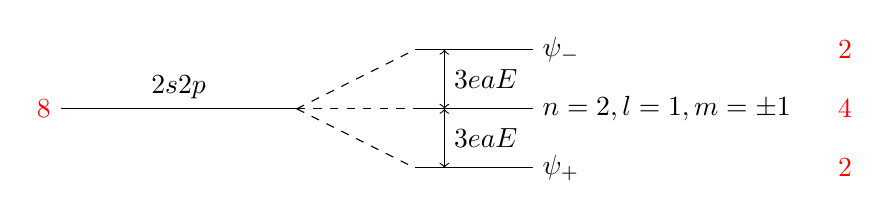
\begin{tikzpicture}[scale=1.5]
    \draw[] (0, 0) -- (2, 0);
    \node[above] at (1, 0) {$2s2p$};
    \draw[dashed] (2, 0) -- (3, 0.5);
    \draw[dashed] (2, 0) -- (3, 0);
    \draw[dashed] (2, 0) -- (3, -0.5);
    \draw[] (3, 0.5) -- (4, 0.5);
    \draw[] (3, 0) -- (4, 0);
    \draw[] (3, -0.5) -- (4, -0.5);
    \node[right] at (4, 0.5) {$\psi_-$};
    \node[right] at (4, 0) {$\ket{n=2, l=1, m = \pm 1}$};
    \node[right] at (4, -0.5) {$\psi_+$};
    \node[left, red] at (0, 0) {$8$};
    \node[right, red] at (6.5, 0.5) {$2$};
    \node[right, red] at (6.5, 0) {$4$};
    \node[right, red] at (6.5, -0.5) {$2$};
    \draw[<->] (3.25, 0.5) -- (3.25, 0);
    \draw[<->] (3.25, 0) -- (3.25, -0.5);
    \node[right] at (3.25, 0.25) {$3eaE$};
    \node[right] at (3.25, -0.25) {$3eaE$};
\end{tikzpicture}
\end{document}